\documentclass[12pt,titlepage]{article}
\usepackage[margin=1.25in]{geometry}
\usepackage{graphicx,amsmath,blindtext,minted}

%% Variables definition
\newcommand{\vSubject}{Computer Networking}
\newcommand{\vSubtitle}{GNS3 and OpenVPN Installation}
\newcommand{\vName}{Muhammad Baihaqi Aulia Asy'ari}
\newcommand{\vNIM}{2241720145}
\newcommand{\vClass}{2I}
\newcommand{\vDepartment}{Information Technology}
\newcommand{\vStudyProgram}{D4 Informatics Engineering}

%% [START] Tikz related stuff
\usepackage{tikz}
\usetikzlibrary{svg.path,calc,shapes.geometric,shapes.misc}
\tikzstyle{terminator} = [rectangle, draw, text centered, rounded corners = 1em, minimum height=2em]
\tikzstyle{preparation} = [chamfered rectangle, chamfered rectangle sep=0.75em, draw, text centered, minimum height = 2em]
\tikzstyle{process} = [rectangle, draw, text centered, minimum height=2em]
\tikzstyle{decision} = [diamond, aspect=2, draw, text centered, minimum height=2em]
\tikzstyle{data}=[trapezium, draw, text centered, trapezium left angle=60, trapezium right angle=120, minimum height=2em]
\tikzstyle{connector} = [line width=0.25mm,->]
%% [END] Tikz related stuff

%% [START] Fancy header related stuff
\usepackage{fancyhdr}
\pagestyle{fancy}
\setlength{\headheight}{15pt} % compensate fancyhdr style
\fancyhead{}
\fancyfoot{}
\fancyfoot[L]{\thepage}
\fancyfoot[R]{\textit{\vSubject - \vSubtitle}}
\renewcommand{\footrulewidth}{0.4pt}% default is 0pt, overline for footer
%% [END] Fancy header related stuff

%% [START] Custom tabular command related stuff
\usepackage{tabularx}
\newcommand{\details}[2]{
    #1 & #2  \\
}
%% [END] Custom tabular command related stuff

%% [START] Figure related stuff
\newcommand{\image}[3][1]{
    \begin{figure}[h]
        \centering
        \includegraphics[#1]{#2}
        \caption{#3}
        \label{#3}
    \end{figure}
}
%% [END] Figure related stuff

%%
\usepackage{pgf-umlcd}

\renewcommand{\umldrawcolor}{black}
\renewcommand{\umlfillcolor}{white}
%%

%% [BEGIN] Custom enumerator
\usepackage{enumitem}
%% [END] Custom enumerator

%% [BEGIN] Paragraph indent
\usepackage{indentfirst}
%% [END] Paragraph indent

%% [BEGIN] URL
\usepackage{hyperref}
\hypersetup{
    colorlinks=true,
    linkcolor=blue,
    filecolor=magenta,      
    urlcolor=cyan,
    pdftitle={Overleaf Example},
    pdfpagemode=FullScreen,
    }

\urlstyle{same}
%% [END] URL

\begin{document}
\begin{titlepage}
    \centering
    \vfill
    {\bfseries\LARGE
        \vSubject\\
        \vskip0.25cm
        \vSubtitle
    }
    \vfill
    
\includegraphics[width=6cm]{images/polinema-logo.png}
    \vfill
    {
        \textbf{Name}\\
        \vName\\
        \vskip0.5cm
        \textbf{NIM}\\
        \vNIM\\
        \vskip0.5cm
        \textbf{Class}\\
        \vClass\\
        \vskip0.5cm
        \textbf{Department}\\
        \vDepartment\\
        \vskip0.5cm
        \textbf{Study Program}\\
        \vStudyProgram
    }
\end{titlepage}

\newpage

\section{Preparation}

\begin{enumerate}
    \item Take notes of the server config, we'll used it later on the tutorial. Open the link to the google drive. \\ \includegraphics[width=.9\textwidth]{images/figures/lmsslc.polinema.ac.id_mod_url_view.php_id=129800.png}
    \item Download the whole google drive folder for the GNS3 and OpenVPN installation setup and OpenVPN profile. \\ 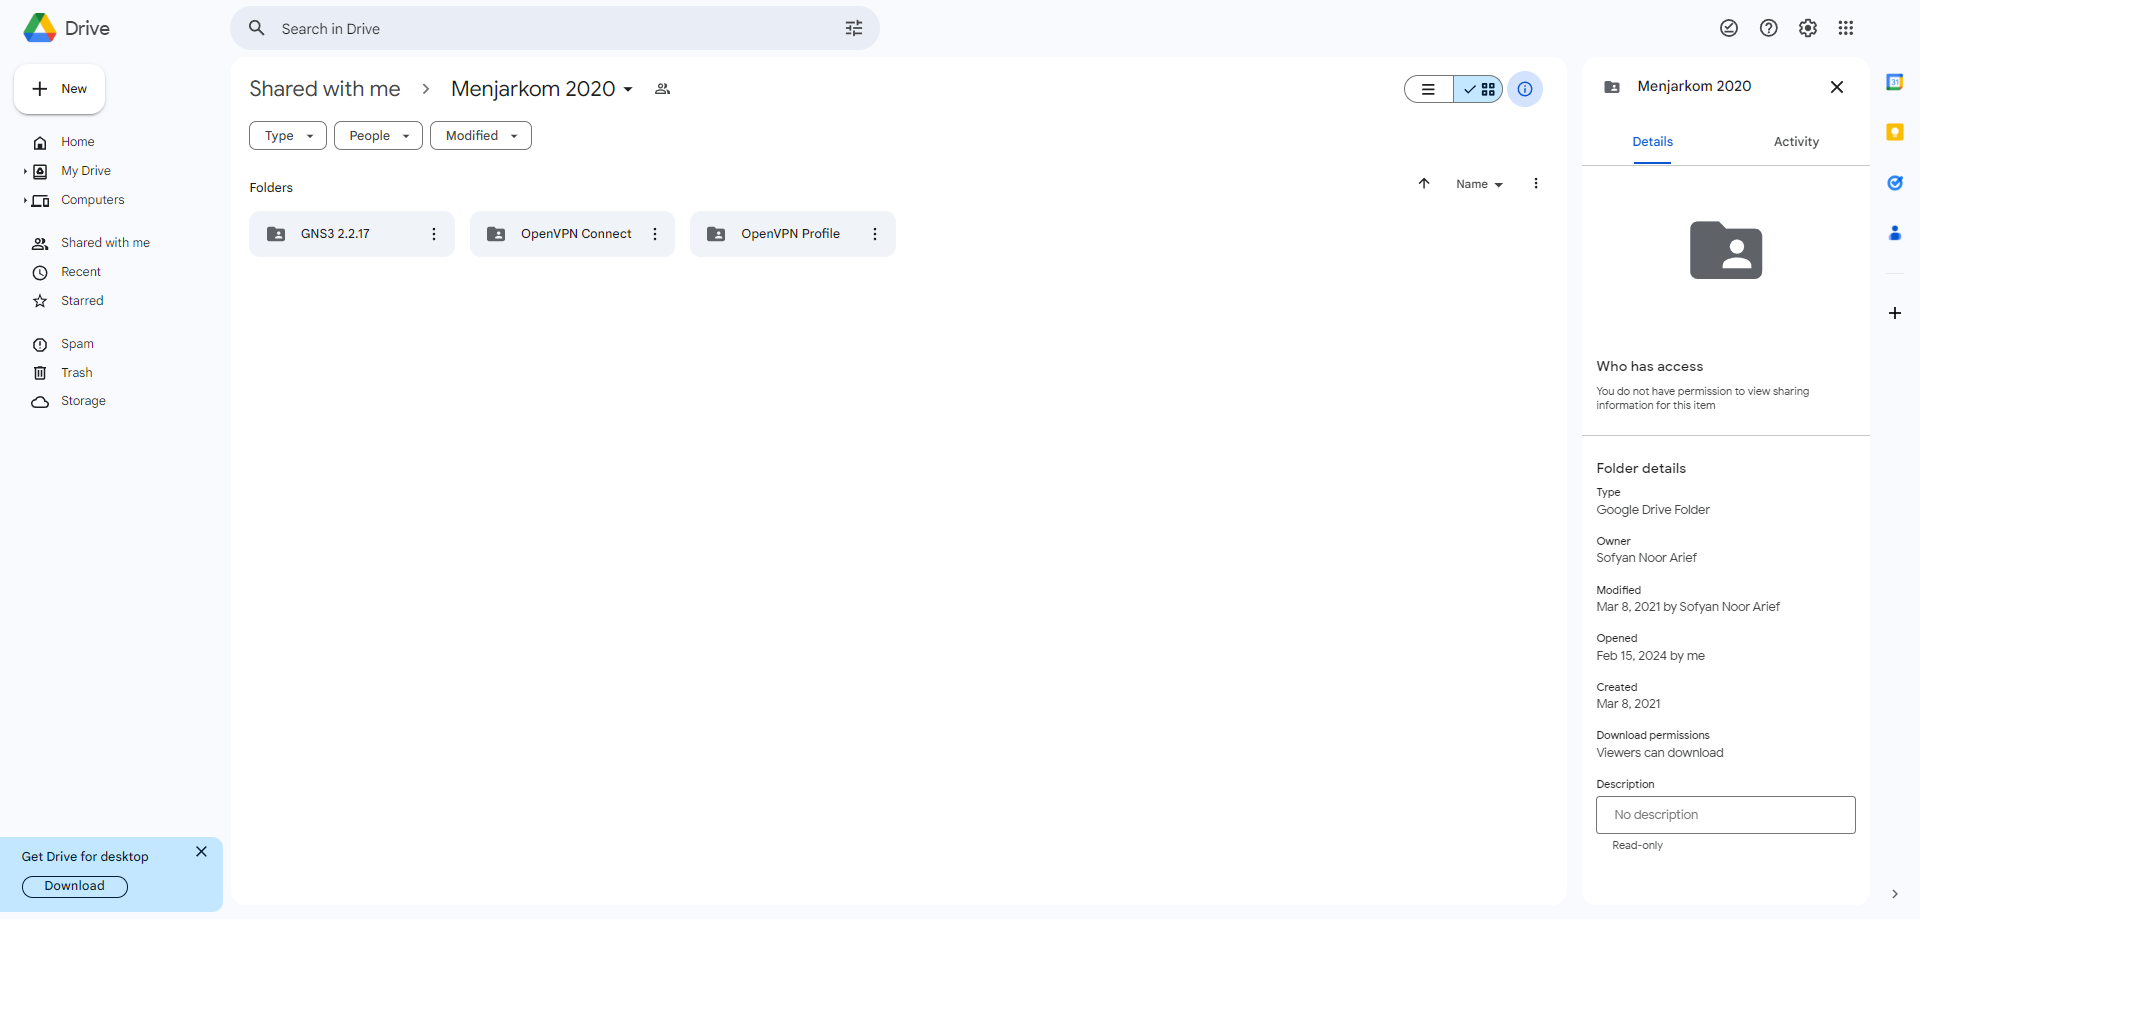
\includegraphics[width=.9\textwidth]{images/figures/drive.google.com_drive_folders_1-SI8APdDK6R4aXmybWSyH4eImjIU0_rt.png}
\end{enumerate}

\newpage

\section{GNS3 Installation}

\begin{enumerate}
    \item Open the GNS3 installation setup folder to the GNS3 installer. \\ \includegraphics[width=.9\textwidth]{images/figures/Screenshot (422).png}
    \item Open the GNS3 installer and click 'next' \\ 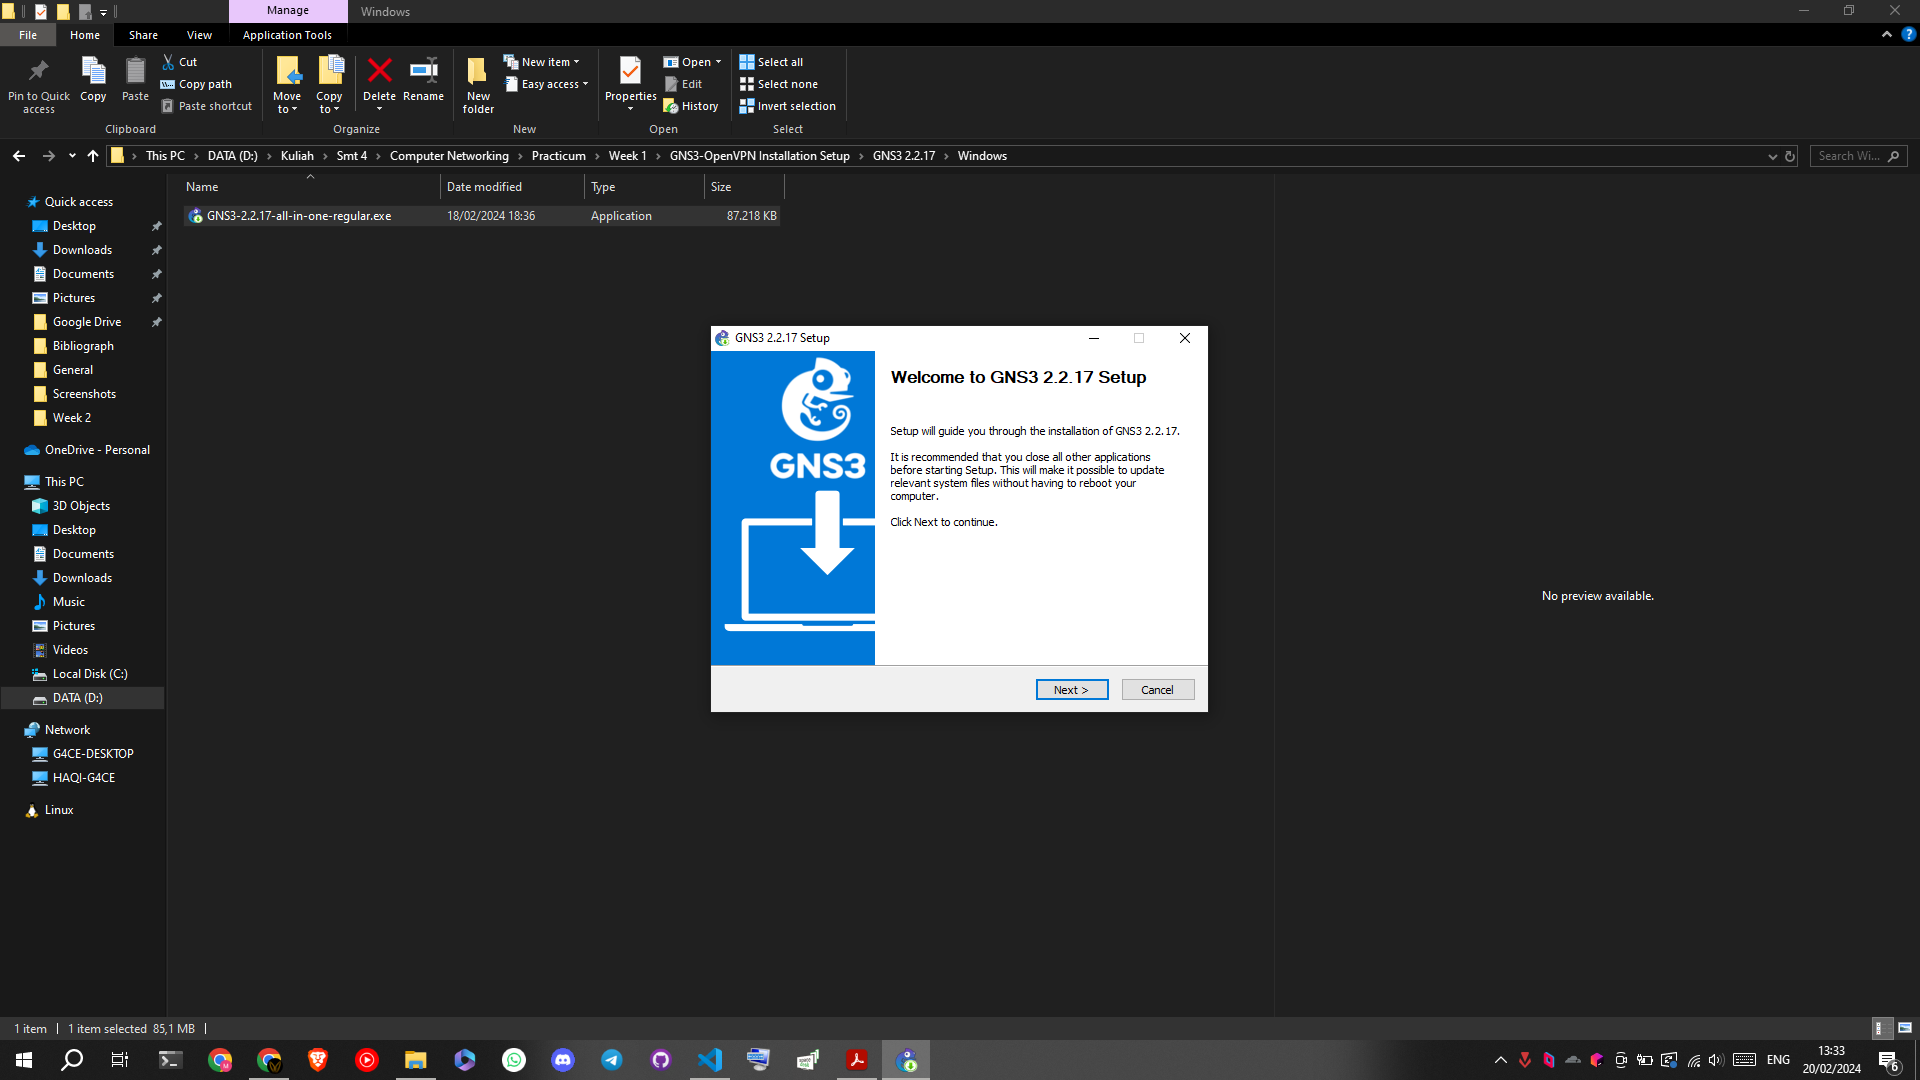
\includegraphics[width=.9\textwidth]{images/figures/Screenshot (423).png}
    \newpage
    \item Click 'I Agree' \\ 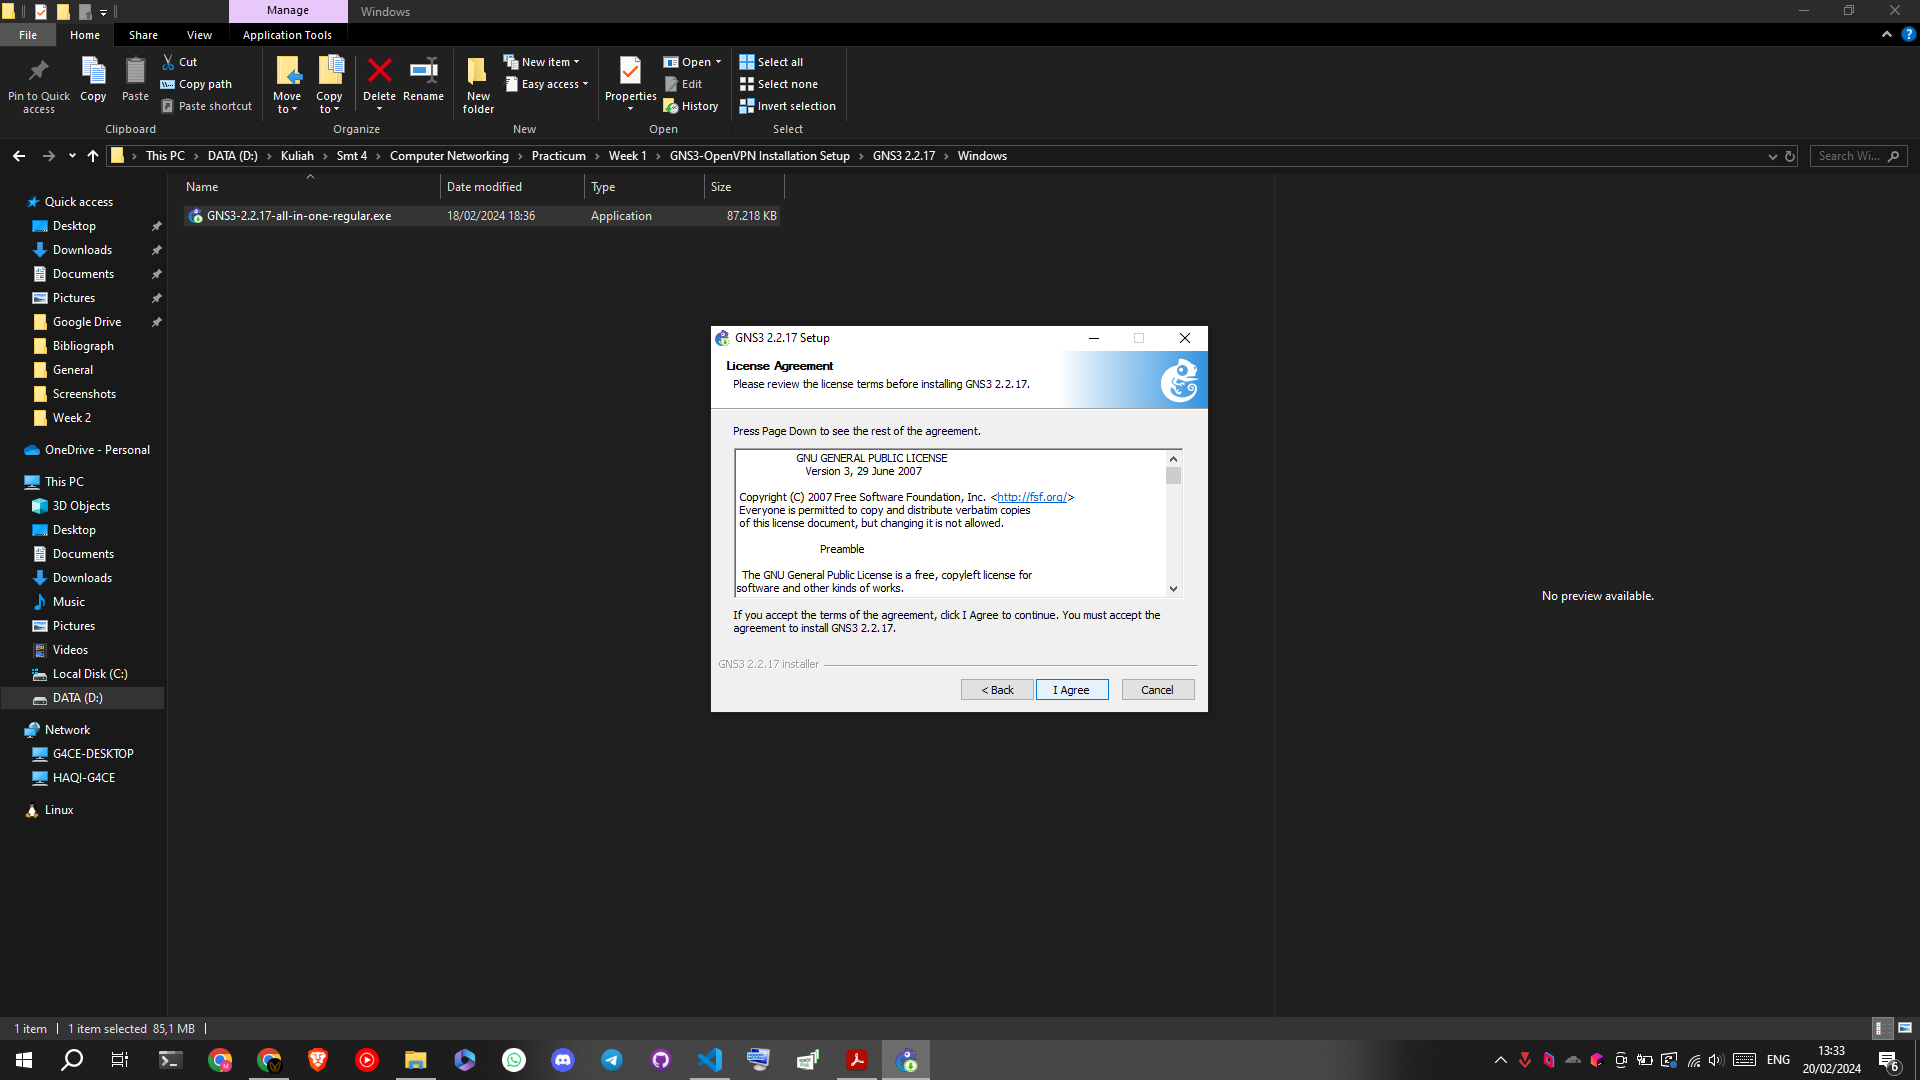
\includegraphics[width=.9\textwidth]{images/figures/Screenshot (424).png}
    \item Click 'next' \\ \includegraphics[width=.9\textwidth]{images/figures/Screenshot (425).png}
    \newpage
    \item Select the desktop and uncheck 'tight-vnc server', 'virt-viewer', and 'solar putty' \\ \includegraphics[width=.9\textwidth]{images/figures/Screenshot (427).png}
    \item Click 'next' \\ 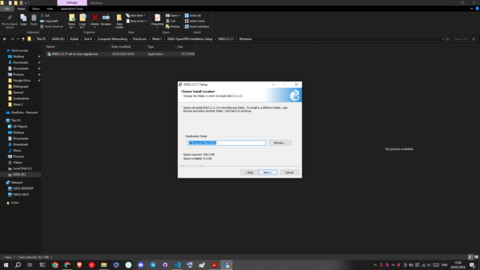
\includegraphics[width=.9\textwidth]{images/figures/Screenshot (428).png}
    \newpage
    \item Wait until further action \\ \includegraphics[width=.9\textwidth]{images/figures/Screenshot (429).png}
    \item Another setup wizard will pop up for WinPcap and Click 'next' \\ 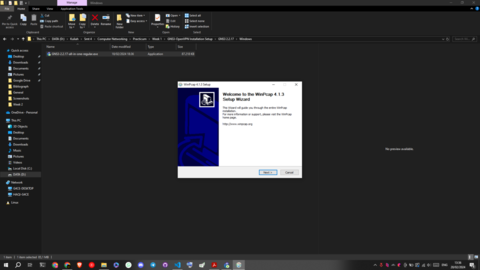
\includegraphics[width=.9\textwidth]{images/figures/Screenshot (430).png}
    \newpage
    \item Click 'I Agree' \\ 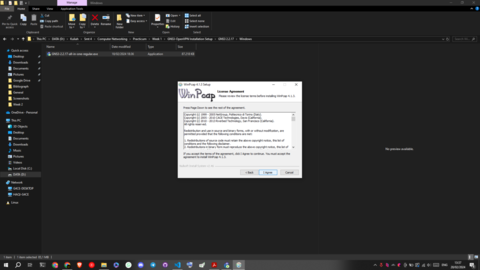
\includegraphics[width=.9\textwidth]{images/figures/Screenshot (431).png}
    \item Click 'Finish' \\ 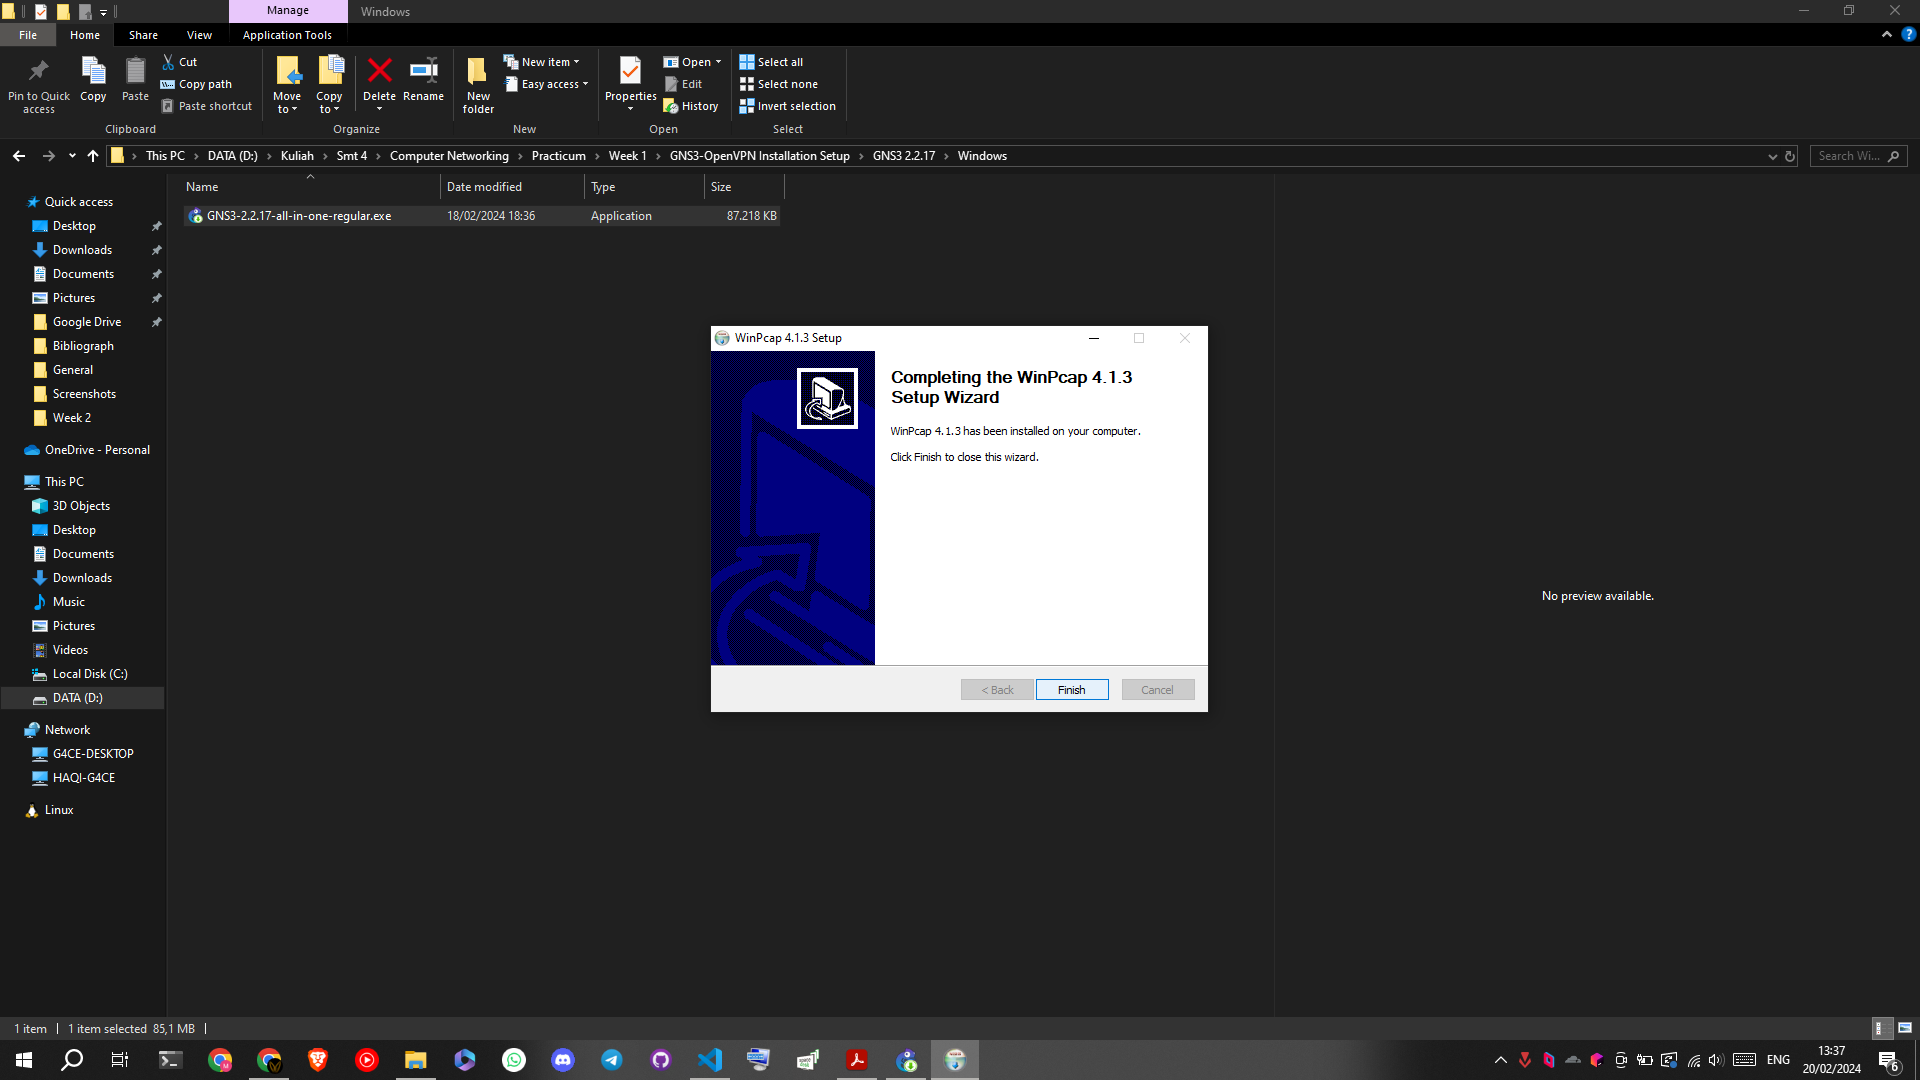
\includegraphics[width=.9\textwidth]{images/figures/Screenshot (432).png}
    \newpage
    \item Another setup wizard will pop up for Npcap and Click 'I Agree' \\ \includegraphics[width=.9\textwidth]{images/figures/Screenshot (433).png}
    \item Click 'Install' \\ \includegraphics[width=.9\textwidth]{images/figures/Screenshot (434).png}
    \newpage
    \item Wait until it's finished \\ \includegraphics[width=.9\textwidth]{images/figures/Screenshot (435).png}
    \item Click 'Next' \\ 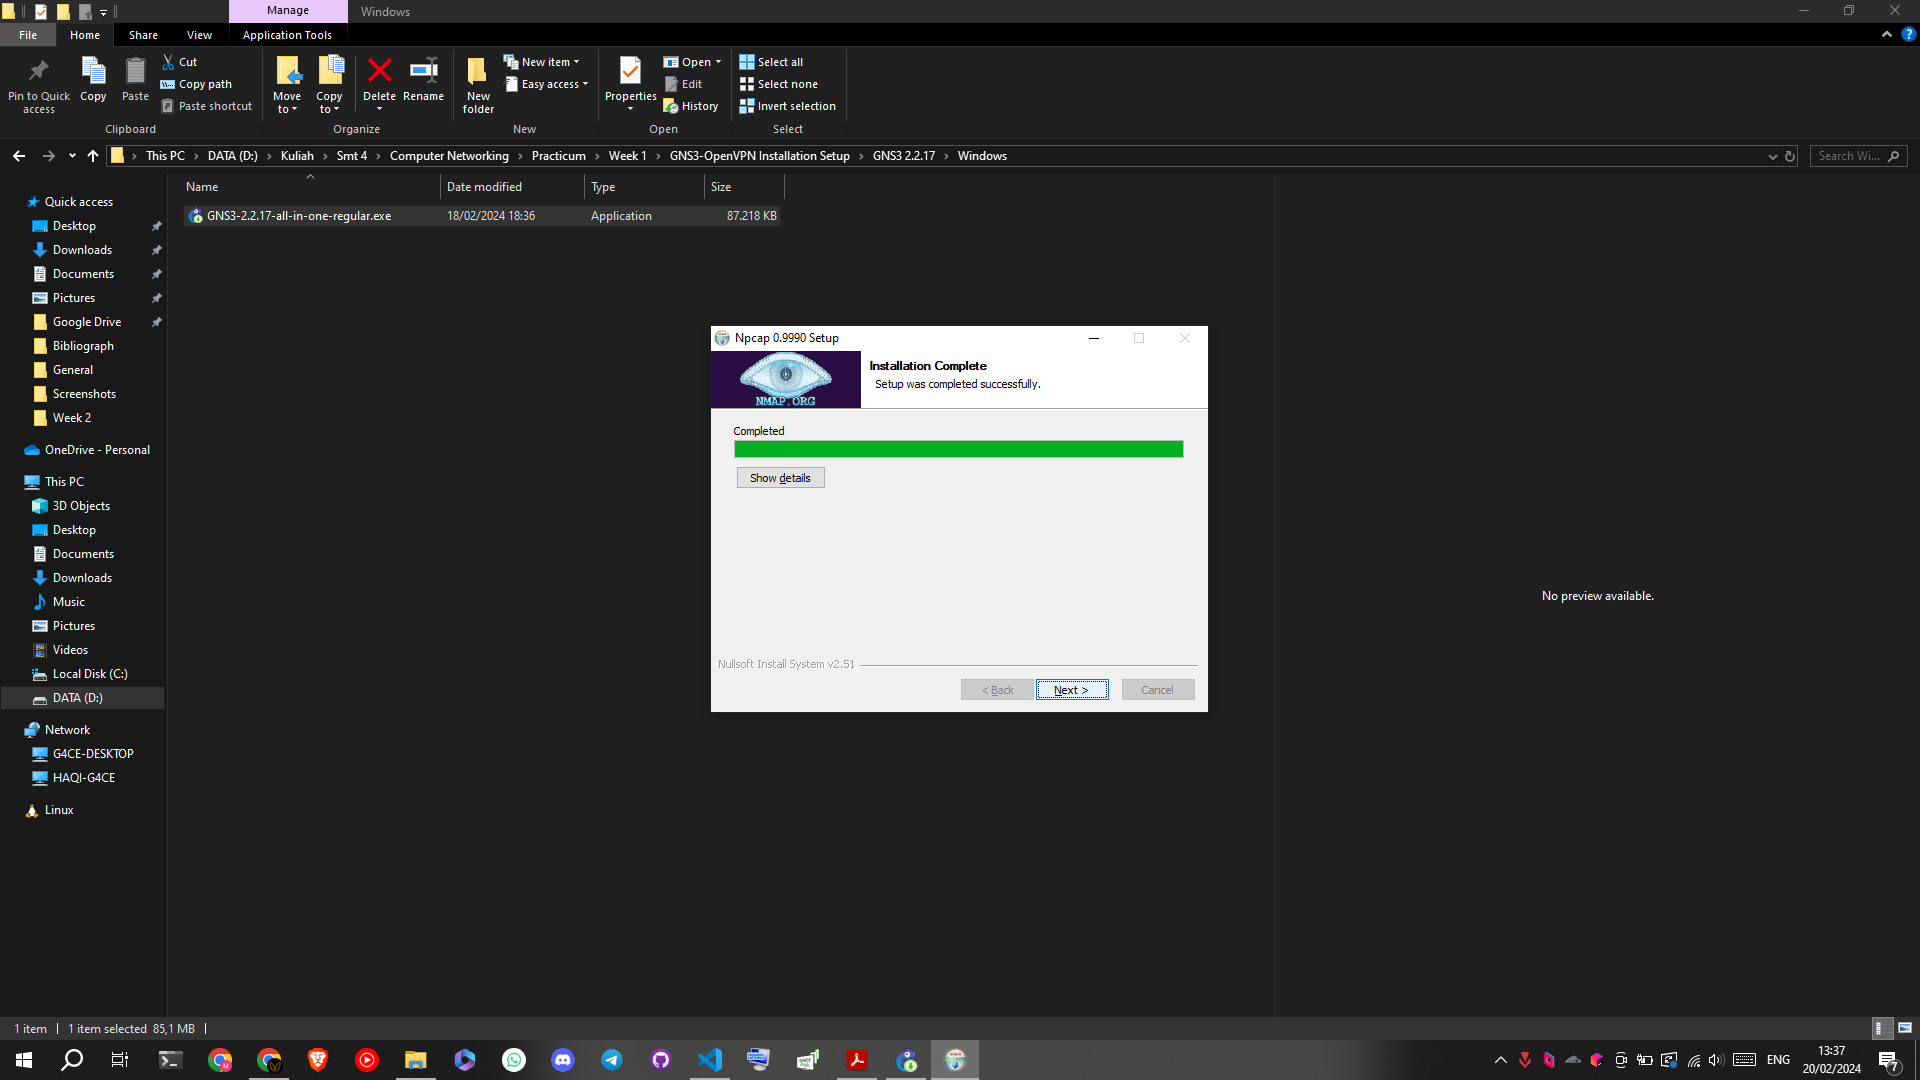
\includegraphics[width=.9\textwidth]{images/figures/Screenshot (436).png}
    \newpage
    \item Click 'Finish' \\ 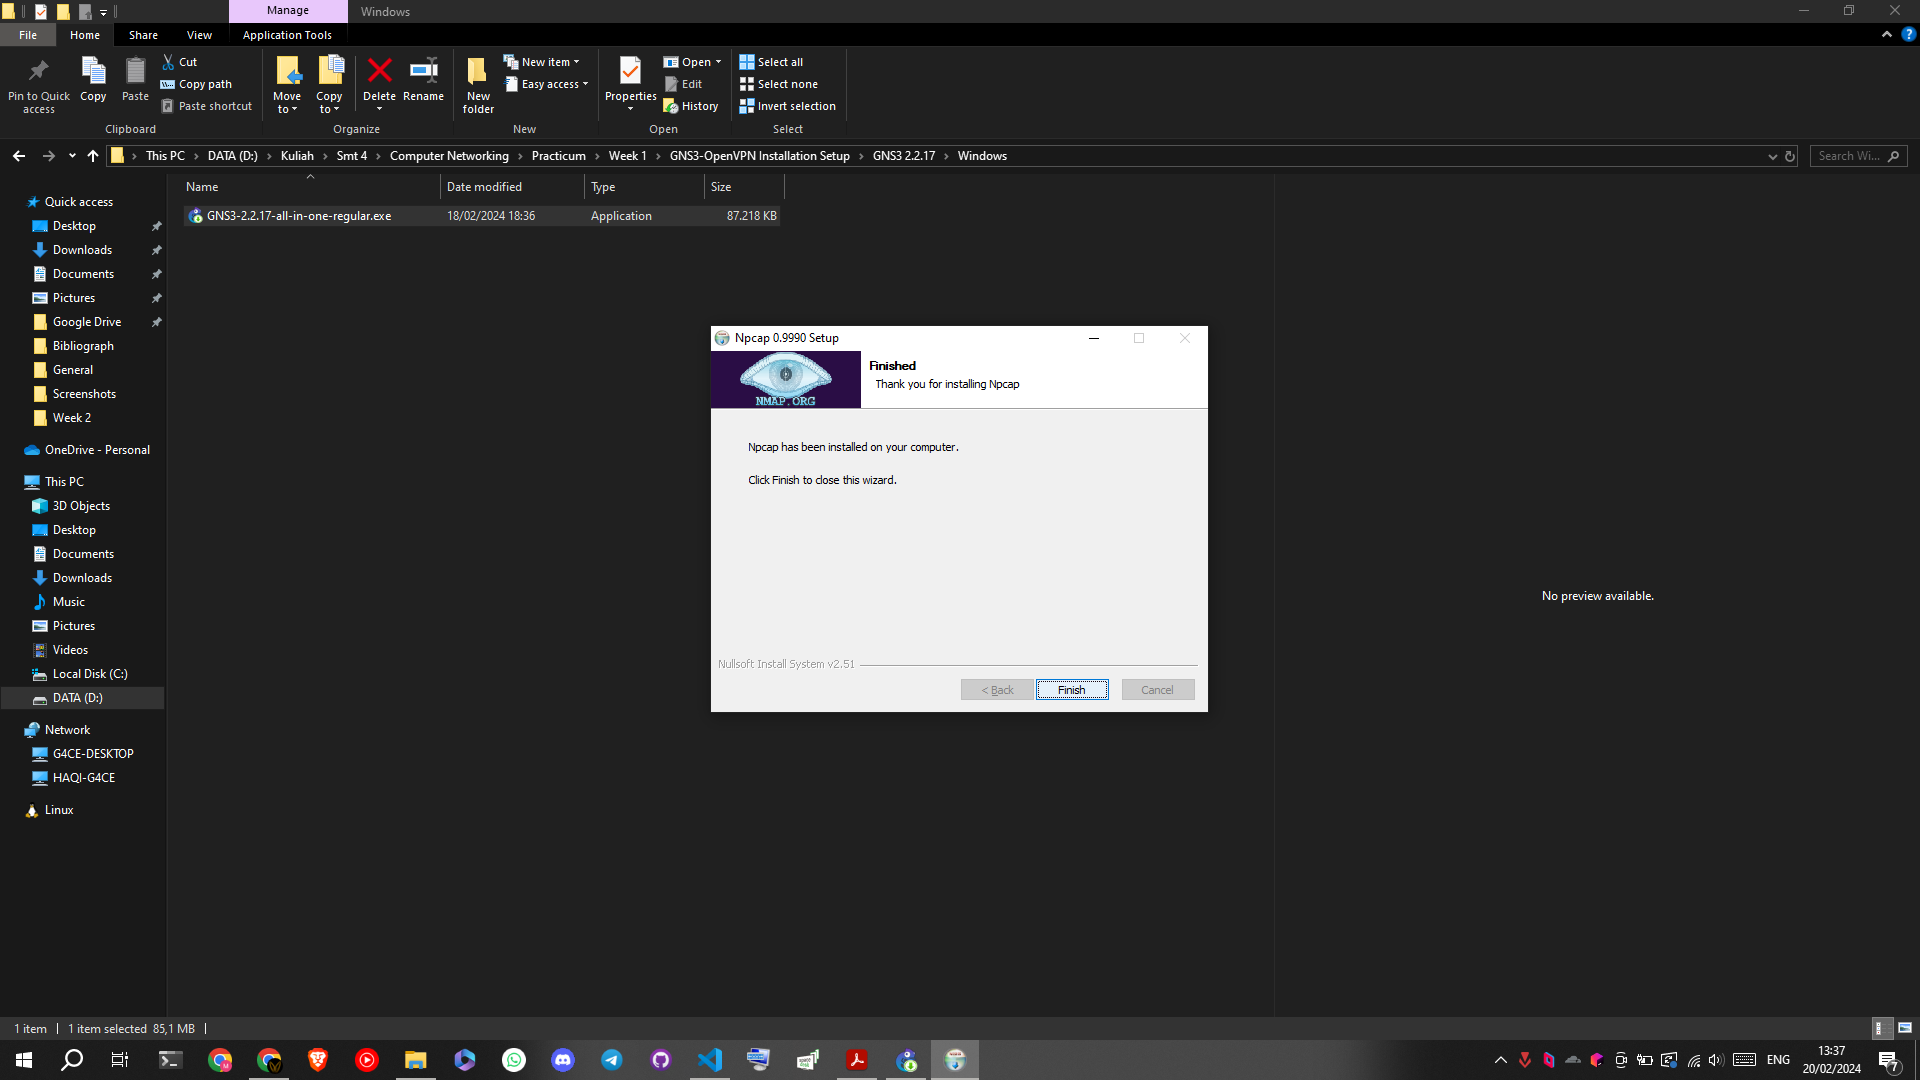
\includegraphics[width=.9\textwidth]{images/figures/Screenshot (437).png}
    \item Wait until it's finished \\ \includegraphics[width=.9\textwidth]{images/figures/Screenshot (438).png}
    \newpage
    \item Click 'Next' \\ 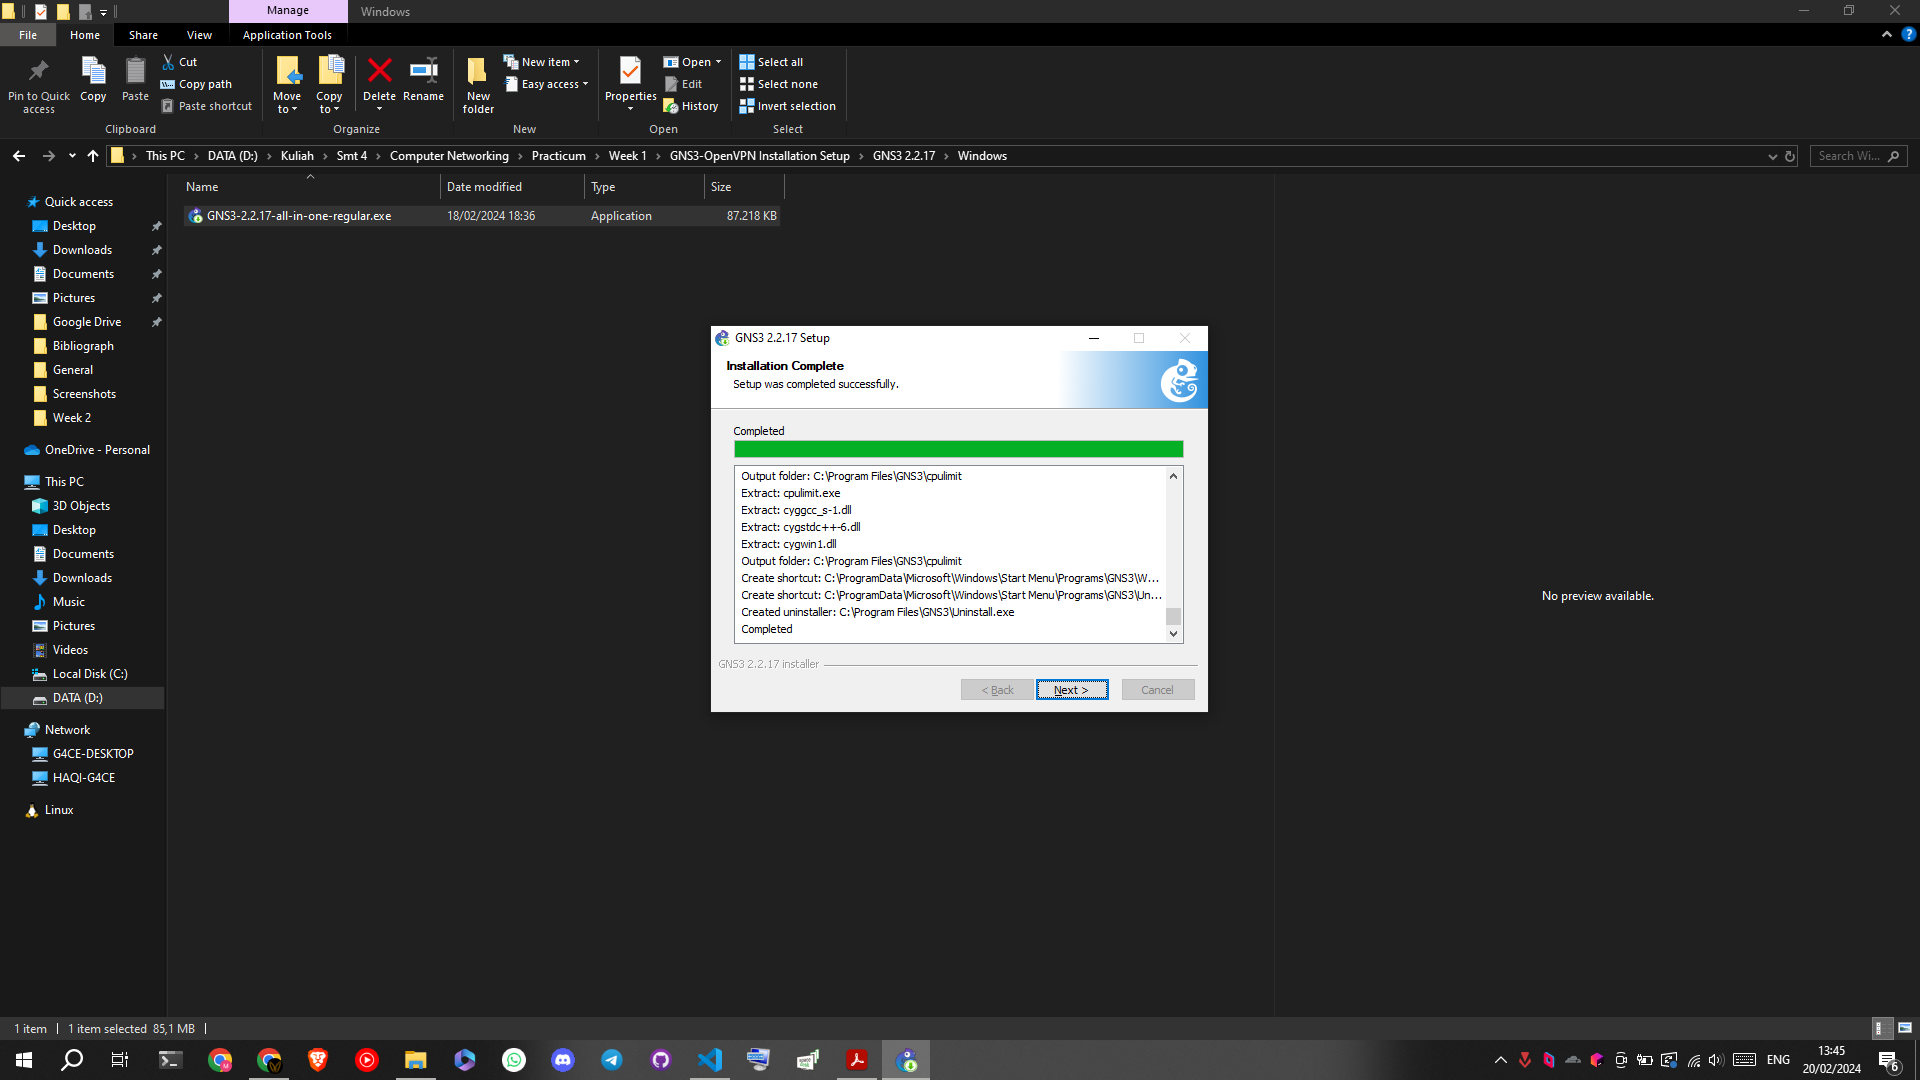
\includegraphics[width=.9\textwidth]{images/figures/Screenshot (439).png}
    \item Click 'No' for Solarwinds Standard Toolset and click 'Next' \\ 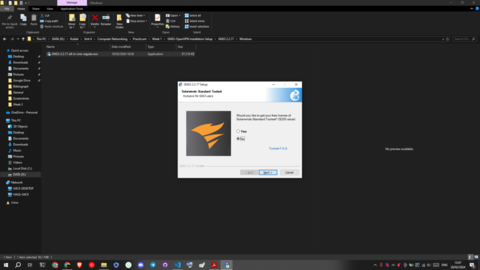
\includegraphics[width=.9\textwidth]{images/figures/Screenshot (440).png}
    \newpage
    \item Uncheck the 'Start GNS3' and Click 'Finish' \\ \includegraphics[width=.9\textwidth]{images/figures/Screenshot (441).png}
    \item Installation finished \\ \includegraphics[width=.9\textwidth]{images/figures/Screenshot (442).png}
\end{enumerate}

\newpage

\section{OpenVPN Installation}

\begin{enumerate}
    \item Open the OpenVPN installation setup folder to the OpenVPN installer \\ 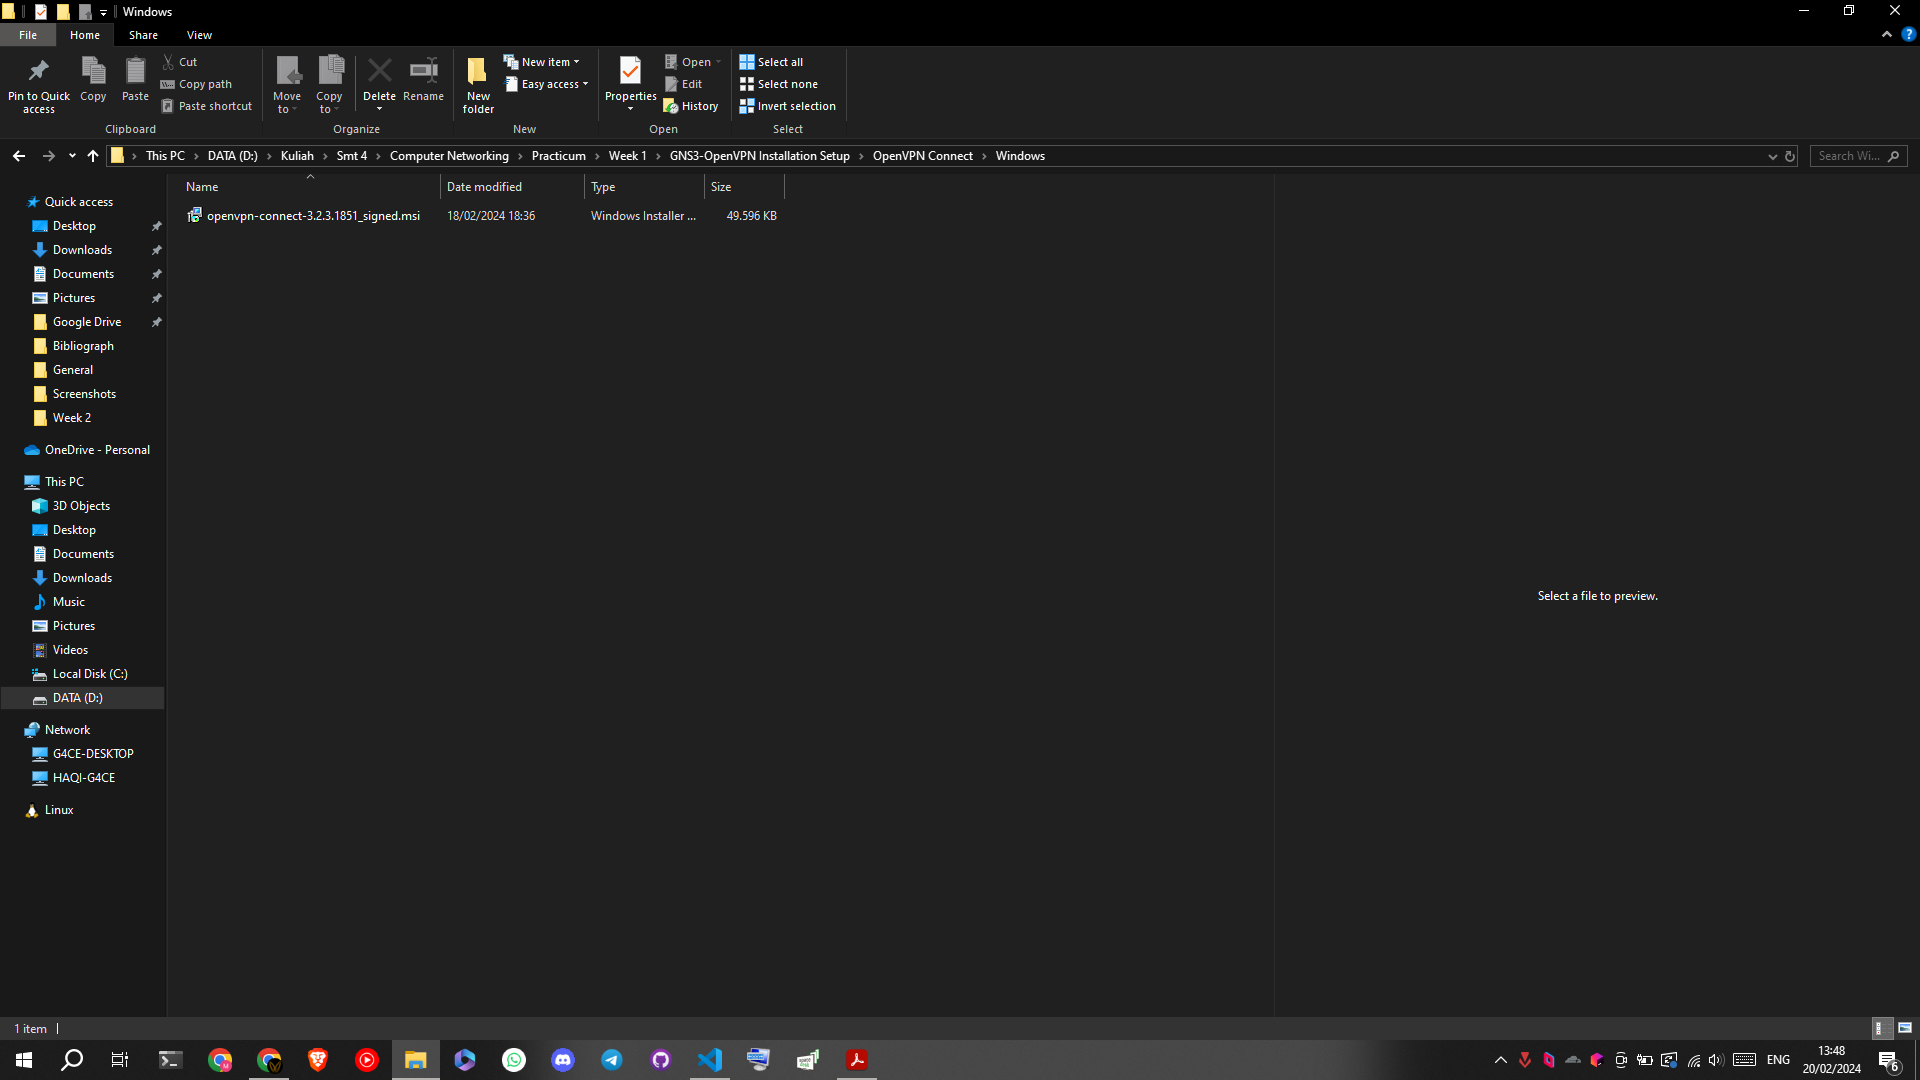
\includegraphics[width=.9\textwidth]{images/figures/Screenshot (443).png}
    \item Open the OpenVPN installer and click 'next' \\ \includegraphics[width=.9\textwidth]{images/figures/Screenshot (444).png}
    \newpage
    \item Checked the 'I accept the terms in the License Agreement' and click 'Next' \\ 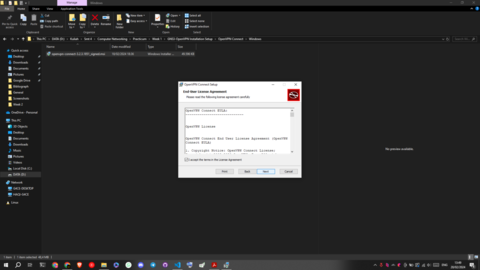
\includegraphics[width=.9\textwidth]{images/figures/Screenshot (445).png}
    \item Click 'Install' \\ 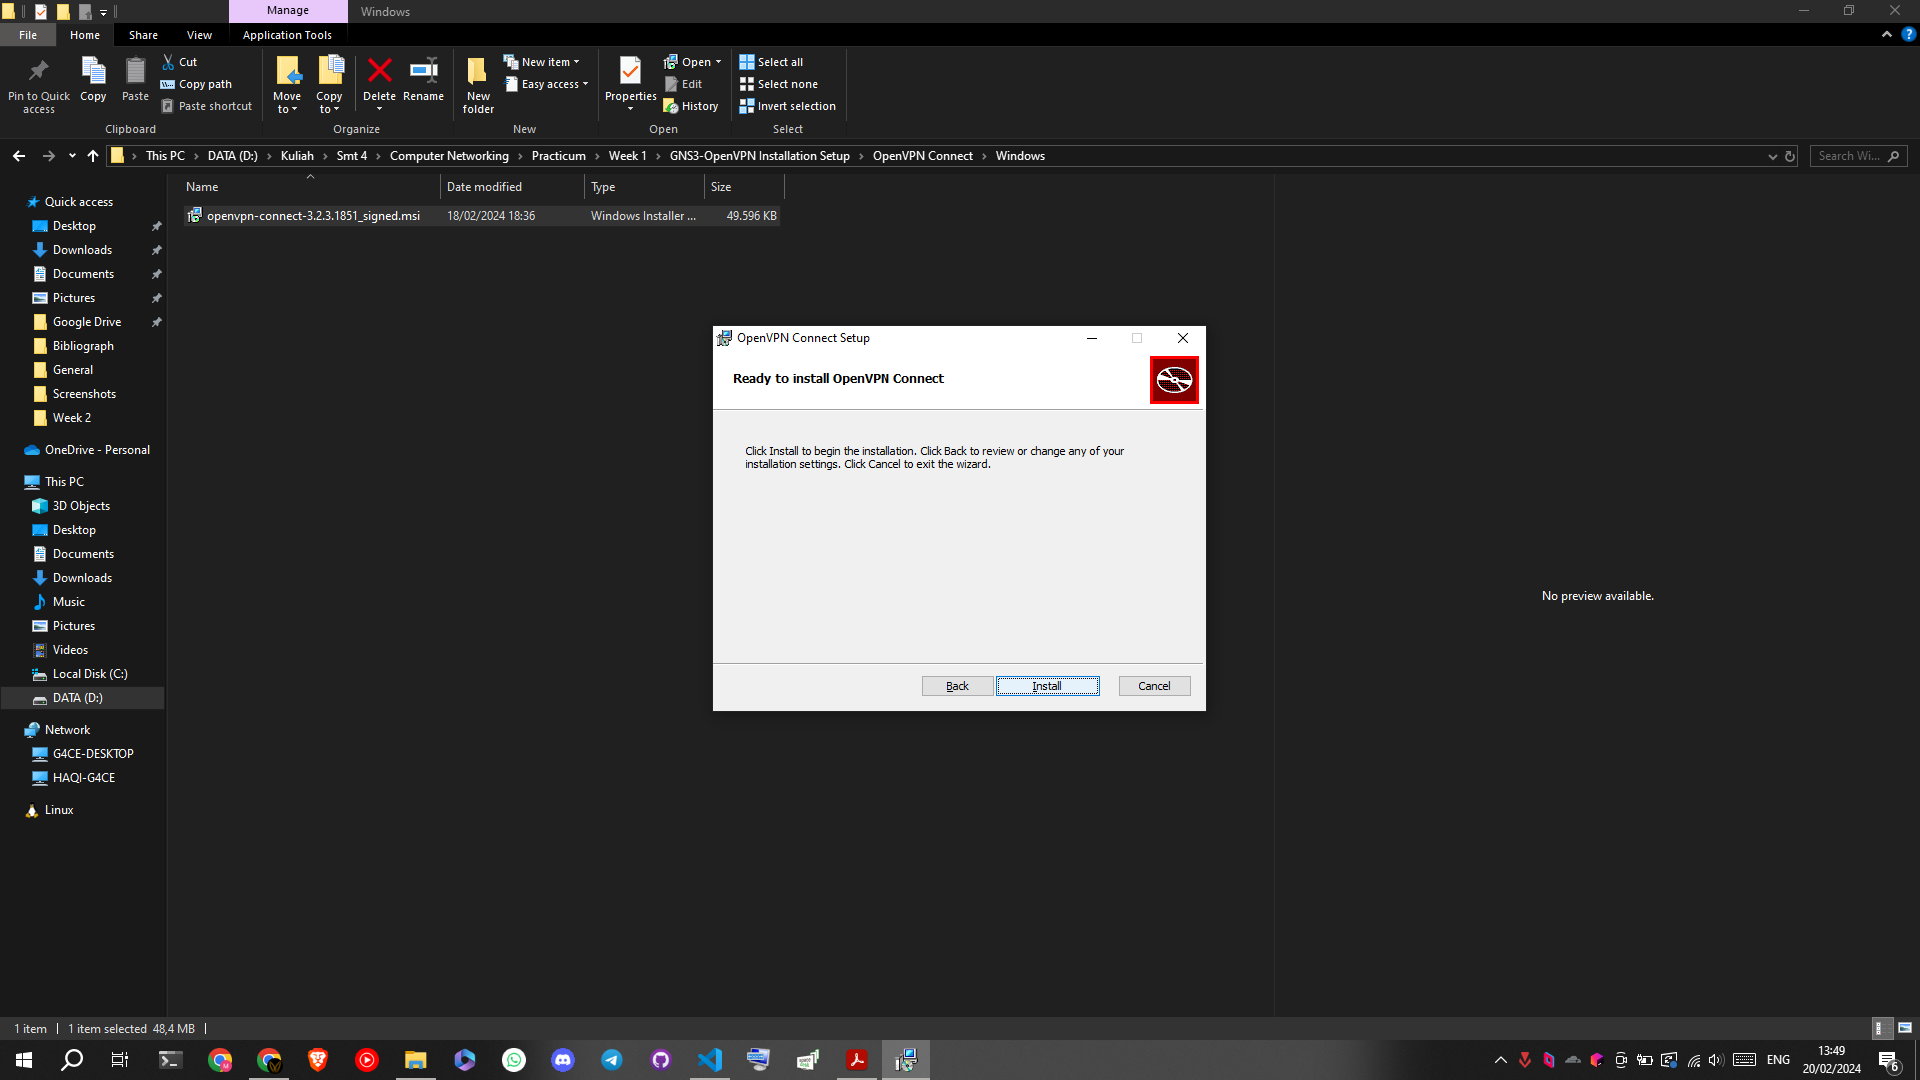
\includegraphics[width=.9\textwidth]{images/figures/Screenshot (446).png}
    \newpage
    \item Wait until it's finished \\ \includegraphics[width=.9\textwidth]{images/figures/Screenshot (447).png}
    \item Click 'Finish' \\ 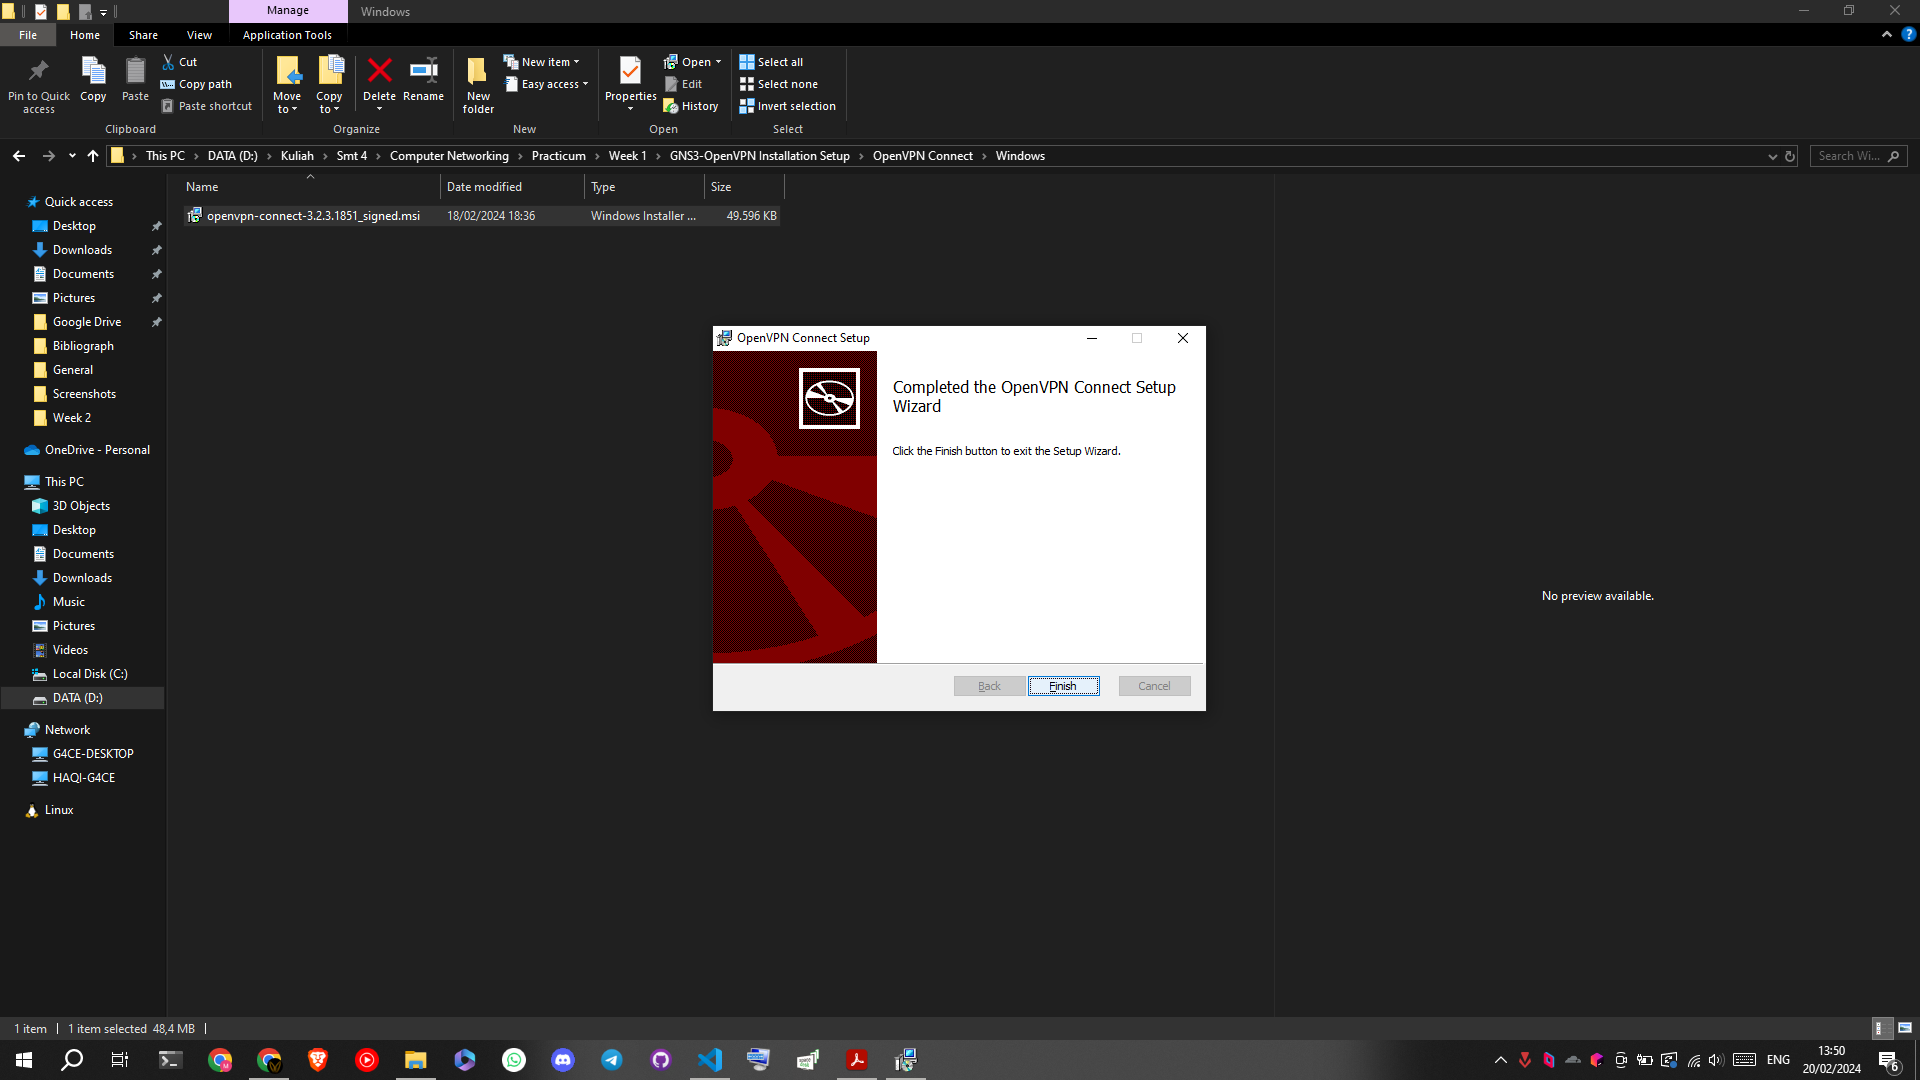
\includegraphics[width=.9\textwidth]{images/figures/Screenshot (448).png}
    \newpage
    \item Open the application and proceed to agree \\ \includegraphics[width=.9\textwidth]{images/figures/Screenshot (449).png}
    \item Click 'OK' \\ \includegraphics[width=.9\textwidth]{images/figures/Screenshot (450).png}
    \newpage
    \item Go to the 'FILE' tab \\ \includegraphics[width=.9\textwidth]{images/figures/Screenshot (451).png}
    \item Click the 'BROWSE' button \\ 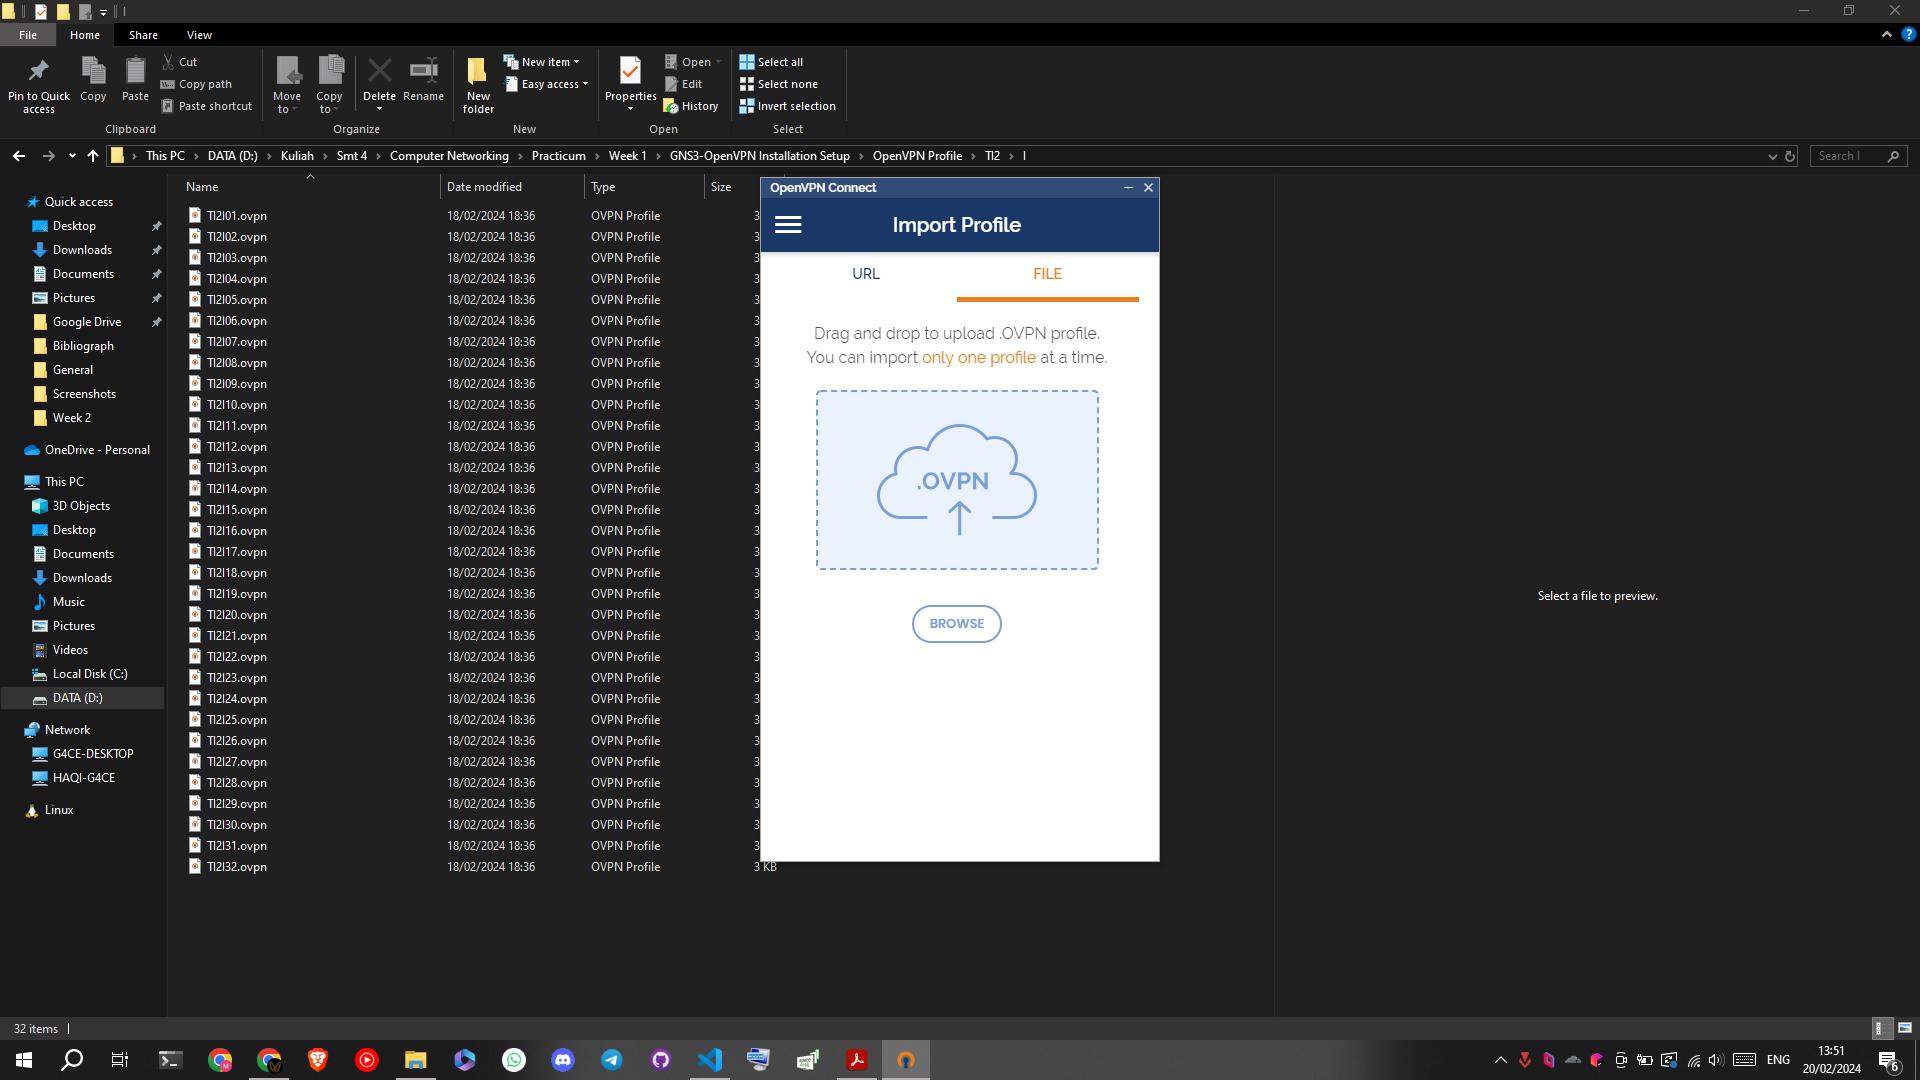
\includegraphics[width=.9\textwidth]{images/figures/Screenshot (452).png}
    \newpage
    \item Select your assigned OpenVPN profile and click 'Open' \\ 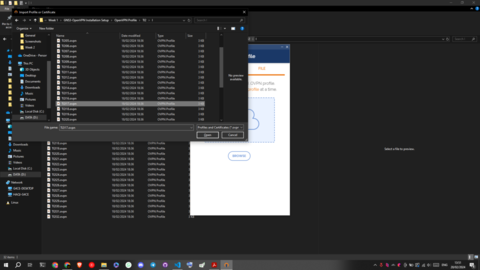
\includegraphics[width=.9\textwidth]{images/figures/Screenshot (453).png}
    \item Click 'Add' on the top right corner \\ 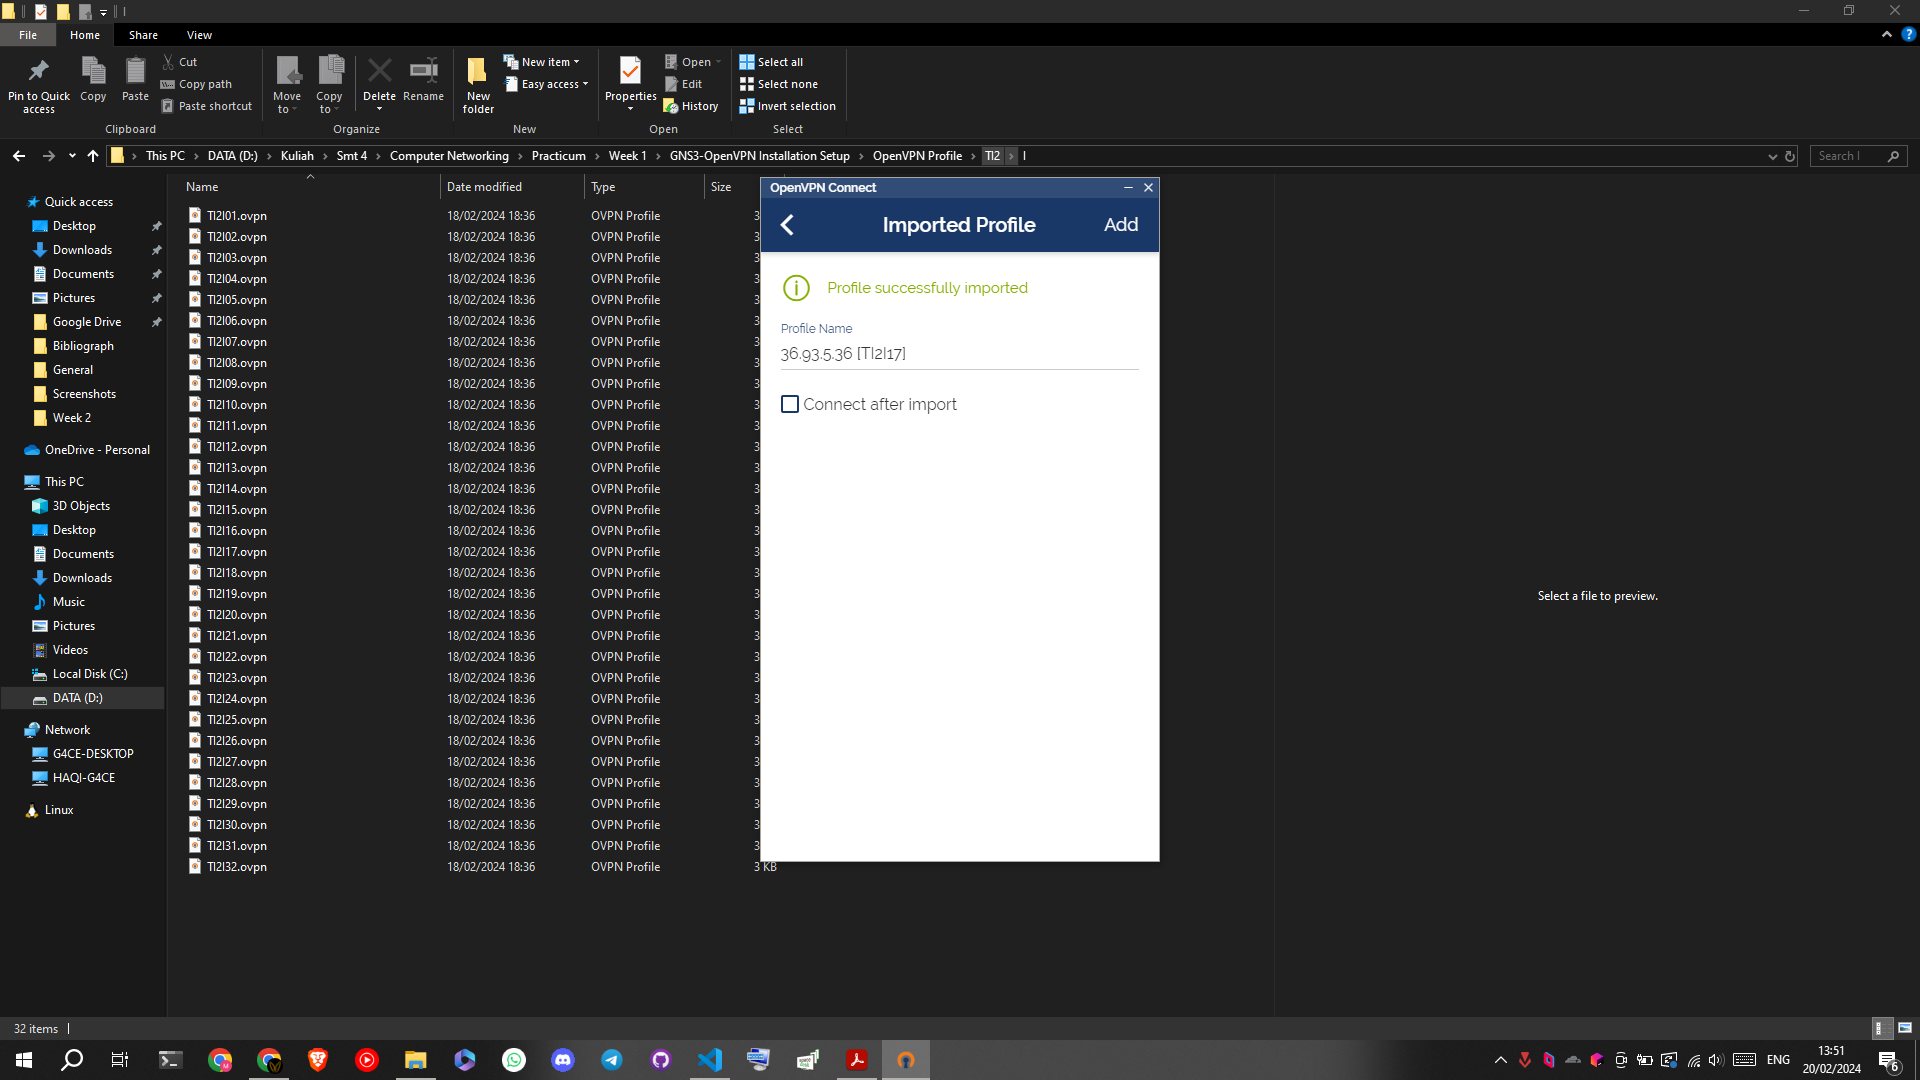
\includegraphics[width=.9\textwidth]{images/figures/Screenshot (454).png}
    \newpage
    \item You can now connect to the campus network by clicking the on/off button of your OpenVPN profile \\ 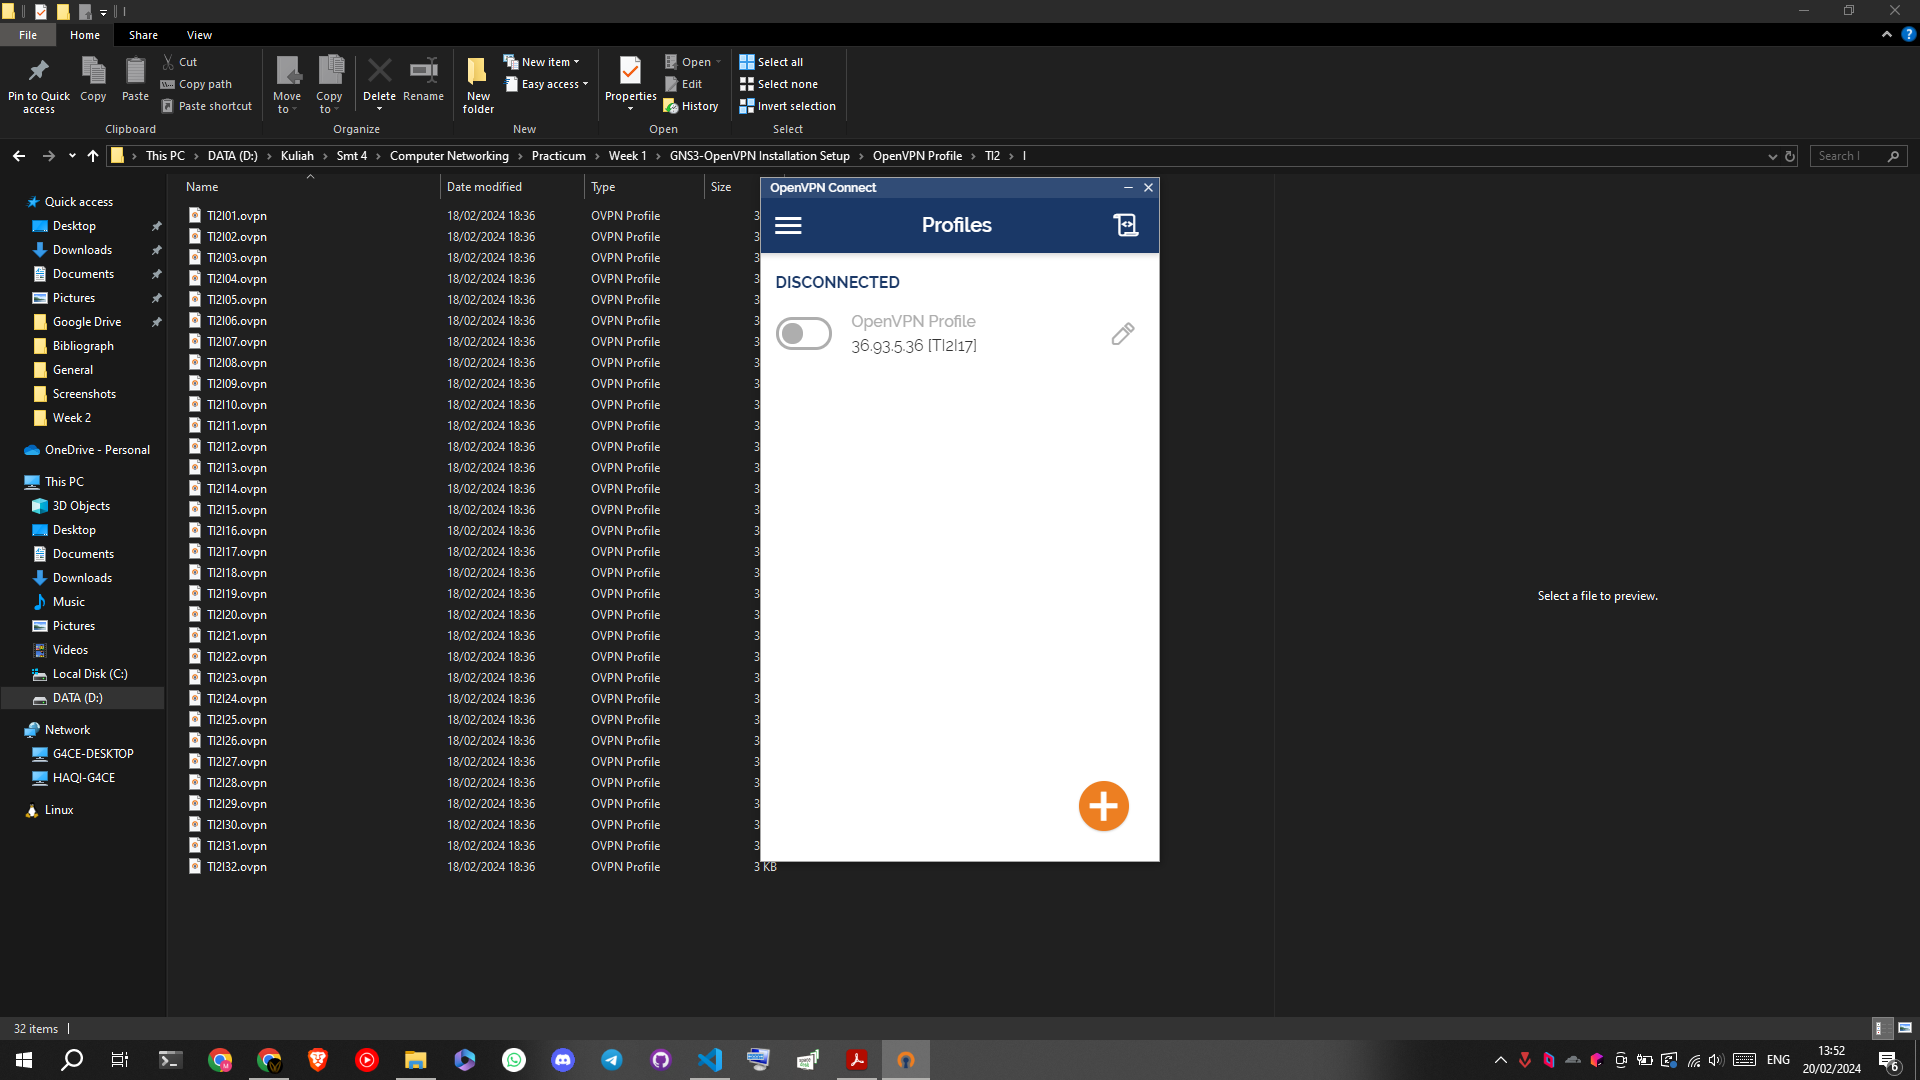
\includegraphics[width=.9\textwidth]{images/figures/Screenshot (455).png}
\end{enumerate}

\newpage

\section{Using GNS3 and Connecting to Server}

\begin{enumerate}
    \item Make sure to connect with the campus network \\ 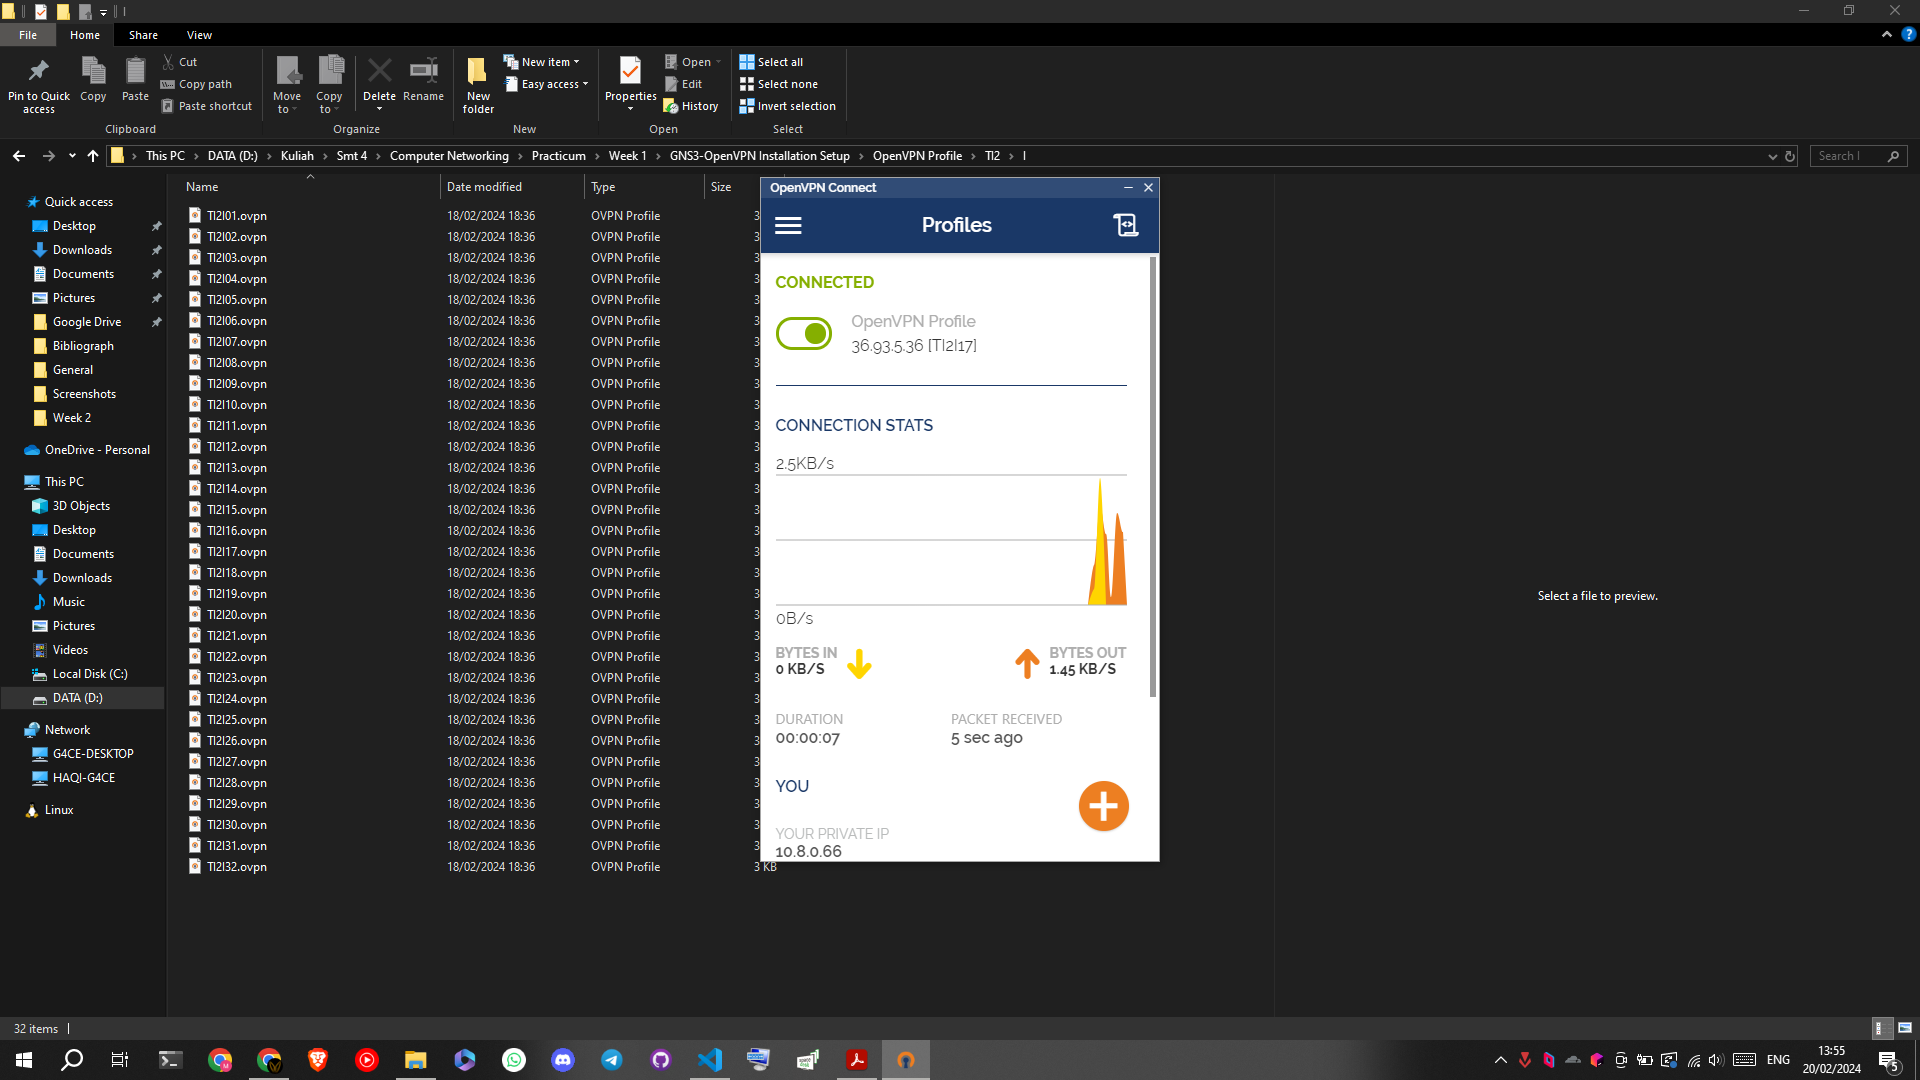
\includegraphics[width=.9\textwidth]{images/figures/Screenshot (456).png}
    \item Open GNS3 and select 'run appliances on remote server' on the intial setup wizard and click 'Next' \\ 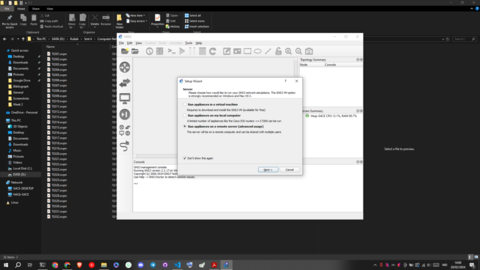
\includegraphics[width=.9\textwidth]{images/figures/Screenshot (458).png}
    \newpage
    \item Insert the previously noted server config and click 'Next' \\ \includegraphics[width=.9\textwidth]{images/figures/Screenshot (459).png}
    \item Click 'Finish' \\ 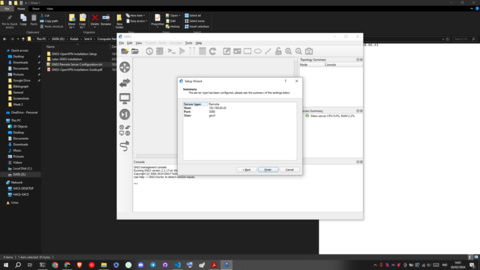
\includegraphics[width=.9\textwidth]{images/figures/Screenshot (460).png}
    \newpage
    \item You can now use GNS3 remotely on campus server \\ 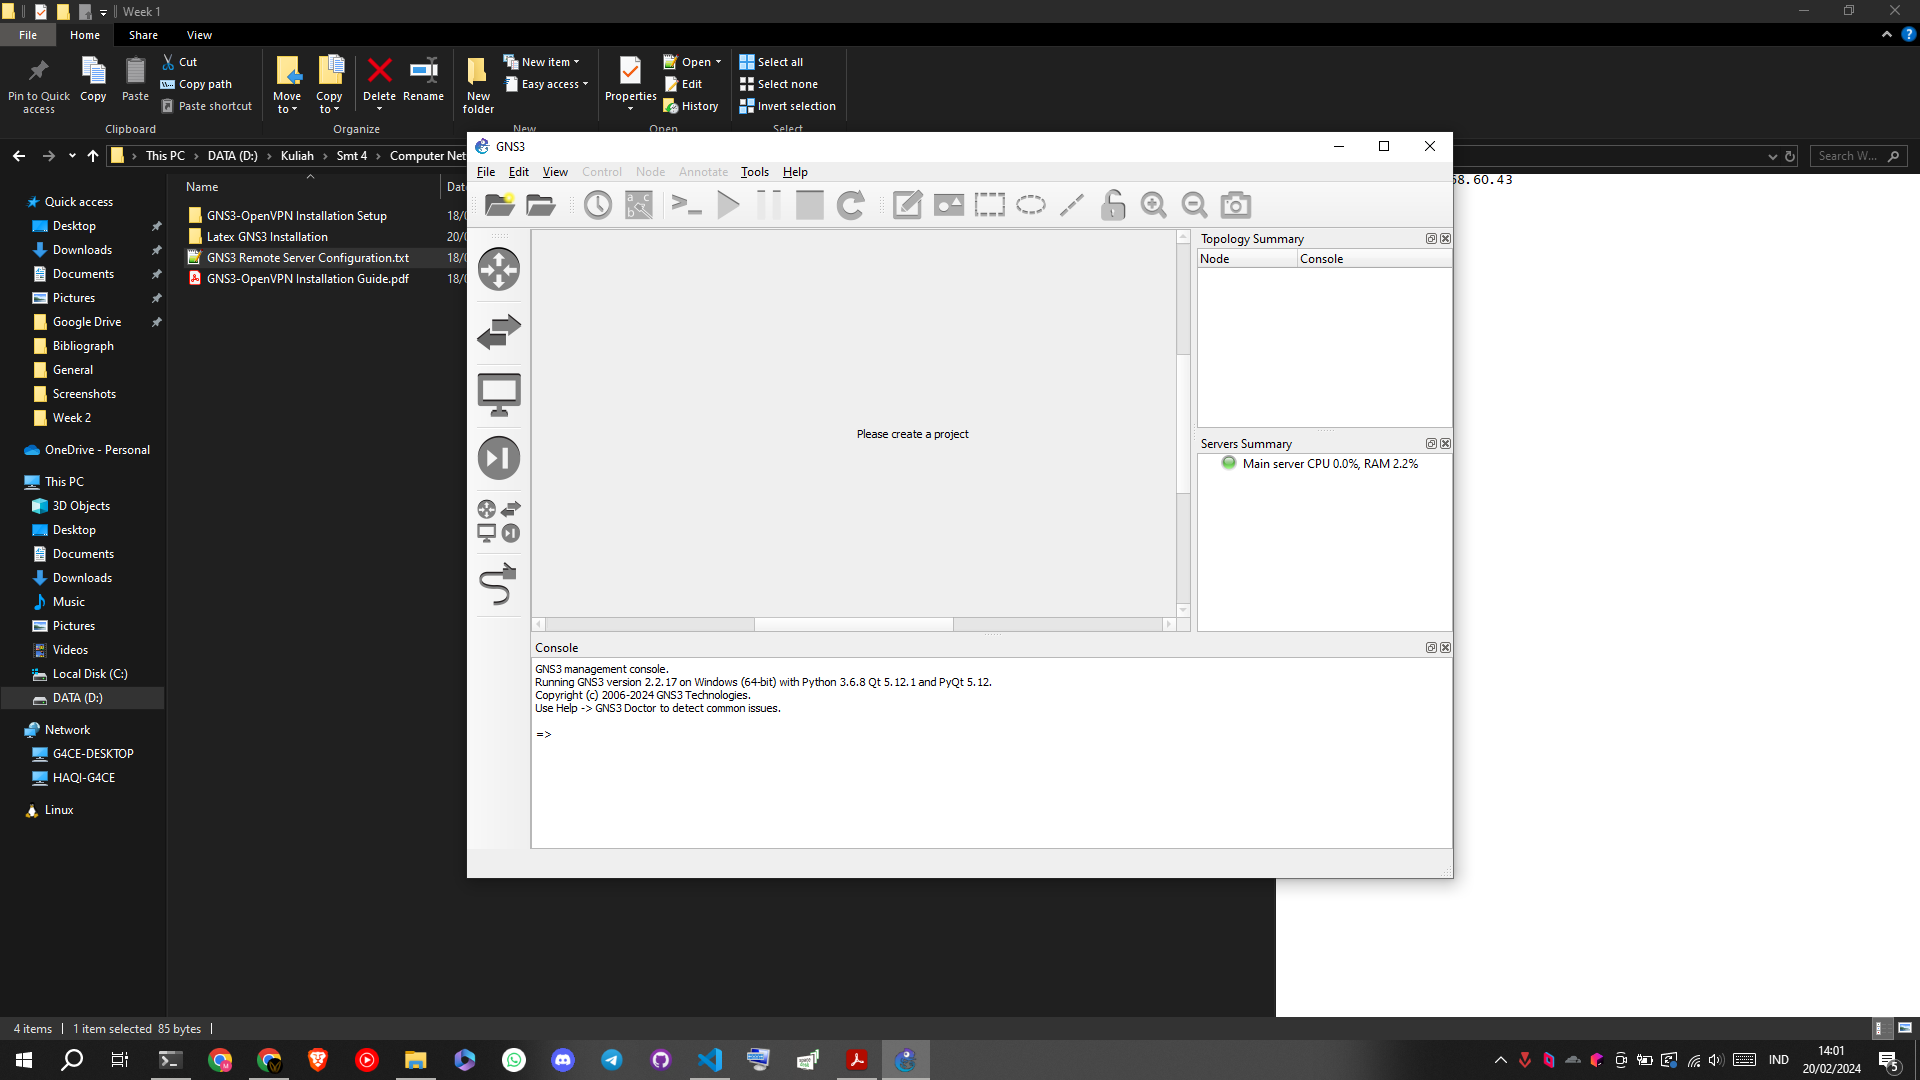
\includegraphics[width=.9\textwidth]{images/figures/Screenshot (462).png}
\end{enumerate}

\end{document}